\documentclass[14pt,twocolumn]{extarticle}

\usepackage[T2A]{fontenc}          
\usepackage[english]{babel}
\usepackage[utf8]{inputenc}

\usepackage{amsmath}
\usepackage{subcaption}
\usepackage{mathtools}
\usepackage{graphicx}
\usepackage{color}
\usepackage{authblk}
\usepackage[colorlinks,citecolor=red,urlcolor=blue,bookmarks=false,hypertexnames=true]{hyperref}
\usepackage{geometry}
\geometry{
	a4paper,
	total={170mm,257mm},
	left=30mm,
	top=20mm,
}

\title{Информационный поиск\\ Индексирование коллекции BY.WEB}
\author{Алфёров Василий, Швецова Анна, Казначеев Дмитрий}

\begin{document}

\maketitle

\begin{abstract}
    Во втором задании мы экспериментировали с Elasticsearch — самым популярным на текущий момент открытым поисковым движком. Elasticsearch основан на Apache Lucene — поисковой библиотеке для Java, корни которой уходят в 1999 год. Elasticsearch предоставляет инструменты для построения индексов и быстрому поиску по нему. В то время как в нём есть встроенная поддержка удаления HTML-тегов и морфологической обработки, этот процесс устроен максимально прозрачно: контент перед попаданием в индекс фильтруется. Это позволяет сделать свою реализацию любого из этих процессов, вставив фильтр на своей стороне.
\end{abstract}

\section{Введение}

В то время как Elasticsearch предоставляет удобный способ заводить и хранить индексы и делать поиск по ним, морфологические фичи предоставлены внешними библиотеками и могут быть реализованы самостоятельно.

В задании от нас требовалось:

\begin{itemize}
\item Проиндексировать коллекцию, замерить время обработки и размер индекса.
\item Произвести морфологическую обработку данных. На каждый способ мы заводили по отдельному индексу, чтобы проще сравнивать результаты.
\item Сравнить результаты поиска по разным метрикам.
\item Добавить PageRank, сравнить результаты с другой обработкой.
\end{itemize}

\section{Первичная обработка данных}

Весь описываемый процесс происходит в \href{https://github.com/vasalf/hse-web-search-homework/blob/master/1/extract.py}{этом скрипте}.
Скрипт создаёт папку \texttt{extracted} и складывает туда по два файла для каждой страницы: текст и метаинформацию, последняя в формате JSON.
Кроме того, он создаёт отдельный файл для своей первичной статистики и пишет её туда в формате JSON.

\paragraph{Извлечение документов}

Документы лежат в XML-файлах. Для начала, нужно достать их оттуда.

Традиционных подходов к парсингу XML-документов два: DOM и SAX.
Первый проще и мощнее, второй заметно быстрее.
В стандартной библиотеке есть также и третий подход, называемый ElementTree.
Нам не хотелось разбираться с новыми подходами для настолько просто устроенных документов, поэтому мы выбирали между первыми двумя.

Проще всего выбрать DOM, но при этом есть опасность, что целое объектное дерево не поместится в оперативную память.
В таком случае следовало бы выбрать SAX или разобраться с ElementTree/pulldom.

В скрипте эта часть имеет заведённый под неё абстрактный класс — мы специально оставили место под написание SAX-парсера в случае, если самая простая реализация MiniDOM будет слишком ресурсоёмкой.

Эксперимент, однако, показал, что для каждого из десяти документов построенное MiniDOM'ом дерево занимало менее 1.5GiB в оперативной памяти, что при имеющихся у нас вычислительных ресурсах нас более чем устраивало. Соответственно, был оставлен MiniDOM-парсер, как самый простой вариант, не требующий чрезмерных человеческих и вычислительных ресурсов.

После извлечения контента нужно было преобразовать его в строчку. Мы использовали встроенный base64-декодер для получения массива байтов, а дальше перекодировали содержимое из cp1251 в UTF8 через встроенную библиотечку \texttt{codecs}. Причина последнего преобразования в том, что в языке Python гораздо проще работать именно с UTF8-строчками. Да и нам тоже на них приятнее смотреть.

\paragraph{Удаление HTML-разметки}

Мы использовали рекомендованную в тексте задания библиотечку BeautifulSoup.
В документации указан способ прикрутить туда альтернативные парсеры XML. Поскольку реальные данные из интернета вовсе не всегда являются корректными xml-документами, дефолтному парсеру от этих данных стало плохо.
После серии экспериментов мы останосились на \texttt{lxml}, дававшем более чем удовлетворительные результаты.

Из разметки мы извлекли метаинформацию и контент. Метаинформация содержит заголовок страницы, её URL (интересный факт, что не все урлы из коллекции являлись корректными ASCII-строчками), а также список урлов, на которые страница ссылается.

Контент можно доставать из документа, пройдясь по всем текстовым узлам, которые достал BeautifulSoup.
Однако не все узлы подойдут: на страницах есть ещё скрипты и CSS-стили, а также комментарии.
Если скрипты и стили можно отсеять по внешнему тегу, то с комментариями в каком-то смысле вышла беда.
По какой-то причине BeautifulSoup их считает за часть текста, не создавая под них отдельного тега.
Решения, основанные на регулярных выражениях, приводили либо к слишком большому времени обработки страницы, либо не были эффективными и оставляли различные артефакты.
В итоге мы смогли от большинства подобных артефактов избавиться через манипуляцию с параметрами BeautifulSoup, который всё же умеет делать элементы под теги, если правильно его попросить.

\paragraph{Параллелизм}

Обработка гигабайтов данных — непростая задача для питона.
Кроме того, из-за GIL там фактически недоступно многопоточное программирование без выхода в другие языки.
К счастью, первичная обработка идеально параллелится по данным, а значит, использовать многопроцессную архитектуру, по процессу на XML-файл, абсолютно ненакладно.
Мы запускали первичную обработку в 4 процесса и на нашем железе в таком режиме она занимала примерно 18 минут.

\paragraph{Первичная статистика}

Статистика, собранная после первичной обработки, приведена в таблице \ref{primary-stats}.

\begin{table}[h]
\begin{tabular}{|c|c|}
    \hline
        Количество документов                              & 200000 \\
        Средний размер документов в словах                 & 808 \\
        Средний размер документов в байтах                 & 7178 \\
    \hline
\end{tabular}
\caption{Статистика, собранная после первичной обработки}
\label{primary-stats}
\end{table}

Распределение длин документов в словах и в байтах, можно посмотреть на рисунках \ref{primary-length-w} и \ref{primary-length-b}, соотвтетсвенно, а соотношение объёма теста и исходного документа — на рисунке \ref{primary-volfraction}.

\begin{figure}[h]
    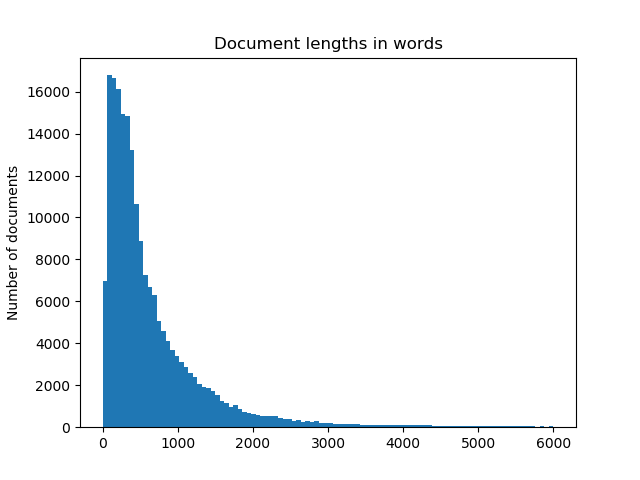
\includegraphics[width=.5\textwidth]{doc_words.png}
\caption{Распределение длин документов в словах}
\label{primary-length-w}
\end{figure}

\begin{figure}[h]
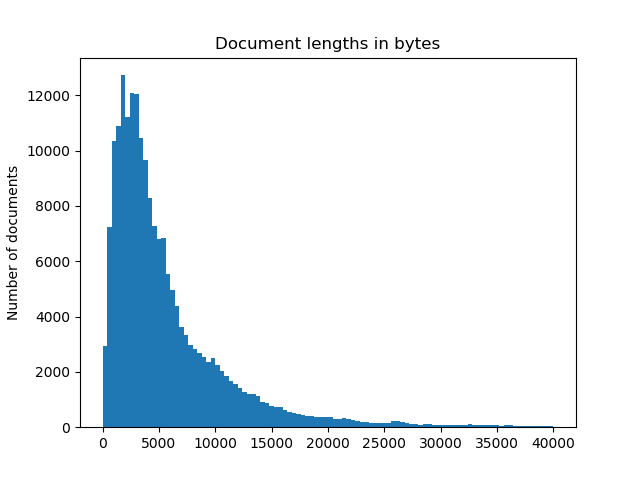
\includegraphics[width=.5\textwidth]{doc_lengths.png}
\caption{Распределение длин документов в байтах}
\label{primary-length-b}
\end{figure}

\begin{figure}[h]
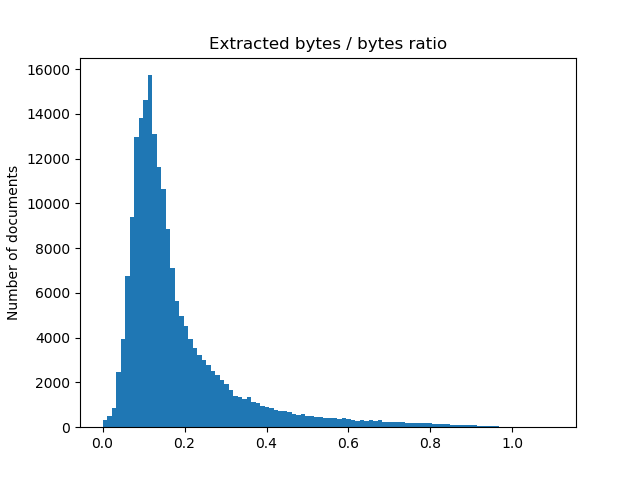
\includegraphics[width=.5\textwidth]{doc_ratio.png}
\caption{Распределение отношения объёмов текста и исходного документа}
\label{primary-volfraction}
\end{figure}


\section{Оценка качества поиска}

Тут Дима, и, вероятно, Аня (??)


\section{Построение и визуализация графа гиперссылок}
\paragraph{}
Процесс построения графа является одним из этапов конвеера обработки и происходит в \href{https://github.com/vasalf/hse-web-search-homework/blob/master/1/pipeline/graph_builder.py}{этом скрипте}. Скрипт создаёт в папке \textbf{result} файлы \textbf{graph\_full.gml} и \textbf{graph\_top.gml}. В файлах в формате GML (Graph Modelling Language) содержатся описания целого графа гиперссылок и подграфа из 150 наиболее популярных страниц.
\paragraph{Построение графа}

Этап построения графа является этапом конвеера обработки данных.

 При инициализации, создаётся пустой ориентированный граф, ассоциативные массивы из URL в целочисленные индексы и обратно, а так же пустое множество обработанных URL обработанных страниц. Для работы с графами использована библиотека \textbf{networkx}, выбранная из-за удобства создания и изменения графа и наличия графовых алгоритмов, в т.ч. PageRank.
 
 На этапе обработки веб-страницы на конвеере мы принимаем выделенную на предыдущем этапе метаинформацию о странице $i$, в которой содержится URL страницы и список URL всех гиперссылок со страницы. URL страницы нормализуется с помощью библиотеки \textbf{urllib}, добавляется в множество обработанных страниц, и ему присваивается уникальный индекс $p_i$. 
 
 Затем каждая гиперссылка $j$ со страницы нормализуется с помощью \textbf{urljoin} относительно базового URL страницы, и из полученного URL убираются все URL-фрагменты. К примеру, на странице \texttt{http://tut.by} гиперссылка \texttt{/index.php\#top} преобразуется в  \texttt{http://tut.by/index.php}. Затем ей присваивается уникальный индекс $p_j$ и в граф добавляется ребро $p_i \rightarrow p_j$.
 
 На этапе сохранения результата считается, что весь граф собран. Из него выделяется подграф на вершинах, являющихся обработанными страницами, таким образом, все внешние ссылки удаляются. Затем из него удаляются все вершины со степенью 0.
 
  Получившийся граф сериализуется в формат GML и сохраняется в \textbf{result/graph\_full.gml}. После этого на нём запускается алгоритм PageRank, и  в \textbf{result/graph\_top.gml} сохраняется подграф на 150 вершинах с максимальным рейтингом PageRank.
 \paragraph{Результаты}
 В итоговом графе содержится 165149 вершин и 1007123 рёбер. Компонент слабой связности всего 4192. В подграфе из 150 вершин с максимальным PageRank 150 вершин и 328 рёбер, 22 компоненты слабой связности. 
 \paragraph{Визуализация}
 Для визуализации использовался инструмент \textbf{Gephi}. Для укладки использовался алгоритм Fruchtermann-Reingold. Вершины и ребра раскрашены в соответствии с компонентой слабой связности, размер вершины пропорционален её PageRank. Граф всех вершин можно увидеть на рисунке \ref{graph-all}, топ-150 Pagerank - на рисунке \ref{graph-top} 
 
 \begin{figure}[h]
 	
\includegraphics[width=.5\textwidth]{graph_all.jpeg}
 	\caption{Граф гиперссылок}
 	\label{graph-all}
 \end{figure}
 
 \begin{figure}[h]
 	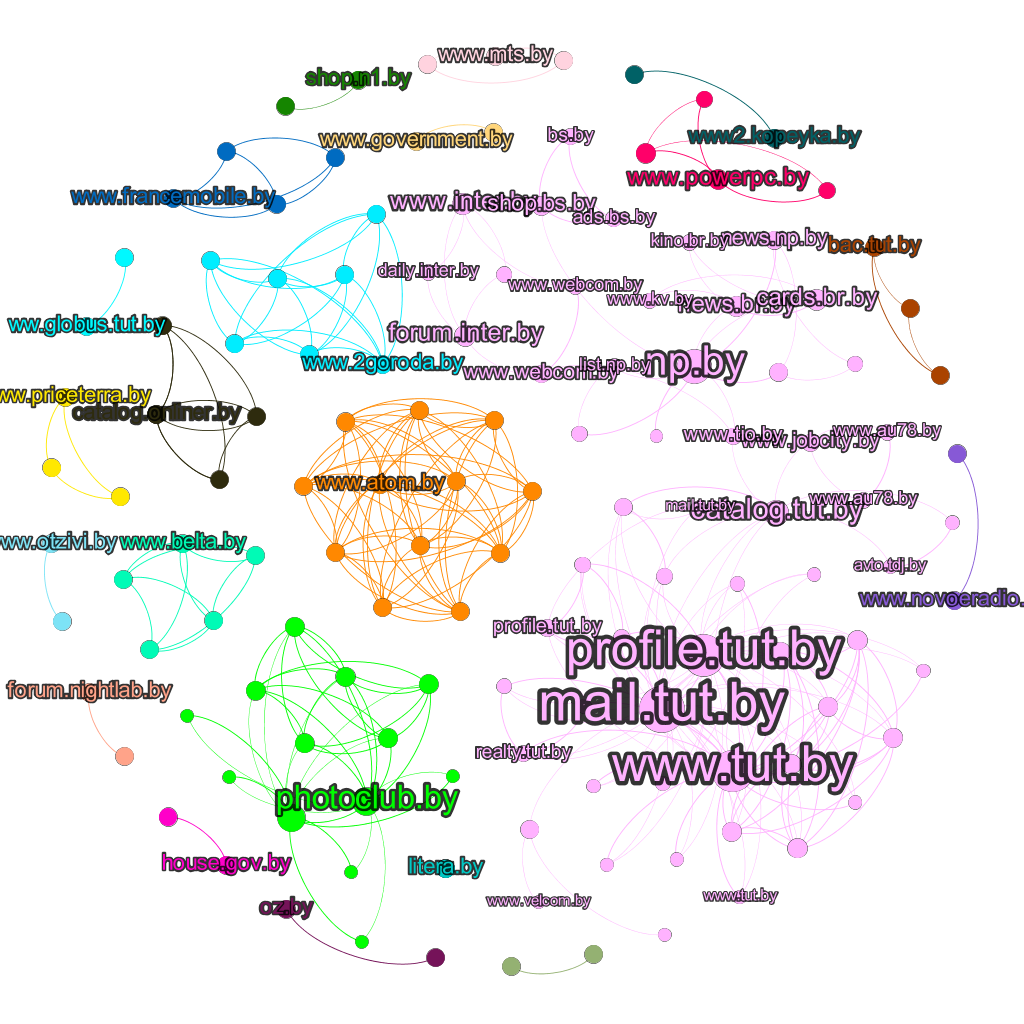
\includegraphics[width=.5\textwidth]{graph_top_white.png}
 	\caption{Граф гиперссылок, топ-150 PageRank}
 	\label{graph-top}
 \end{figure}
 

\end{document}
